\section{Distributed databases}
\label{sec:distributed-dbs}

\subsection{Distributed, decentralized and centralized databases}

\iffalse
- to fully comprehend distributed databases, we have to distinguish them from decentralized and centralized databases. baran 1964: in context of networks: distributed vs centralized and decentralized in between
- apply this definition to databases: add examples: one single database: standard example, decentralized: cloudfront CDN by amazon, distributed: bittorrent
\fi

To understand distributed databases, it is important to distinguish them from decentralized and centralized databases. Baran (1964) \cite{baran-distributed-communications} explains the difference in the context of networks. A centralized network makes all nodes connect to one central node. A distributed network is the opposite, in which any node can communicate with any other node without the need for a central node. In-between lies the decentralized network, in which there are a couple of central nodes that communicate with each other. Other nodes have to connect with one of these central nodes.
Figure \ref{fig:baran-networks} visualizes the differences.

\begin{figure}[h]
\centering
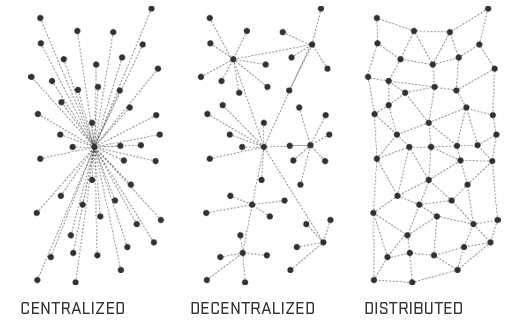
\includegraphics[width=0.8\textwidth]{paper-images/baran_networks.png}
\caption{Baran, P. (1964) Centralized, decentralized and distributed networks.} 
\label{fig:baran-networks}
\end{figure} 

This definition can be ported to the context of databases. A centralized database consists of one main data storage node. Users connect to this node to read and write data. A self-hosted website is a perfect example of a centralized database. Any user that wants to connect to your website, has to connect to your server. If your server breaks down, nobody can access the website anymore.

A decentralized database has many storage nodes that communicate with each other. A user can connect to either of these main nodes to access the data. Use of a CDN (Content Delivery Network) is an example of a decentralized database. Websites hosted on a CDN are copied across servers all over the world. To access to this website, a user can connect to any of these servers.

Finally, a distributed database does not have main storage nodes. Instead, every node can hold the entire database. When a new node wants to access the data, the node asks its peers for the data. Examples are BitTorrent and git, which both will be discussed in section \ref{subsec:examples-distributed-dbs} of this chapter.

\subsection{Consistency, availability, and partition-resilience: the CAP theorem for distributed systems}

Clearly, a trade-off is made when deciding between a centralized or distributed database. When a user reads data from a centralized node, the user receives the correct data, as there is only one version of the data. However, when this one centralized node somehow breaks down, nobody will be able to access the database anymore. Fox and Brewer (1999) \cite{brewers-theorem-paper} calls such a database not ``partition-resilient''. This means that when an arbitrary amount of nodes goes offline in the network, the entire system stops operating.

The opposite is true when working with a distributed database. Even though some nodes are offline, a user can always connect to the data through the other nodes. However, this comes at a drawback. The data the user reads is not necessarily the most updated version, as it could have been updated on another node in the meantime. Fox and Brewer (1999) calls such a database not ``consistent''.

To avoid the consistency issue, a distributed database can force all nodes to update to the most recent version before responding to any more read requests. But it could happen that a connection between a not-updated node and the updated node is broken. This prevents the not-updated node from receiving the latest version of the data. The node will refuse any read requests until the connection is restored, to not provide incorrect information. This node is still online and functioning, but not responding to requests. Fox and Brewer (1999) calls such a database not ``available''.

The CAP theorem (Consistency, Availability, and Partition-resilience) states that any network can choose two out of three characteristics. The theorem was first proposed by Fox and Brewer (1999). It was formally proven by Gilbert and Lynch (2002) \cite{gilbert-lynch-cap-proof}.

\subsection{Issues with distributed databases in collaborative systems}
\label{subsec:issues-distributed-dbs}

In a guided system, there is one authoritative entity controlling every node in the network. But in a collaborative system, separate agents with individual incentives have to work together. This creates a whole new set of challenges, namely consensus and immutability issues.

Consensus issues arise when the database has been updated on two different nodes at the same time. Somehow, these two conflicting versions have to merge. % For example, Alice spends a cryptocurrency coin to buy something from Bob. But at the same time, she uses this same coin to buy something from Claire. etc etc

Immutability issues emerge when the agreed upon past can be changed. For example, Alice wants to spend a cryptocurrency coin. The merchant makes sure that the coin is valid and approves the purchase. But when immutability is not properly enforced, Alice can go into the database and manually remove the transaction. This nullifies the transaction, allowing Alice to spend the coin again.

\subsection{Examples of distributed databases and networks used in collaborative systems}
\label{subsec:examples-distributed-dbs}
% how does every example do on the CAP theorem, what are other disadvantages

The final part of the chapter discusses several common implementations of distributed databases and networks in the context of collaborative systems. 

\subsubsection{Git version control}

Git is the most popular distributed version control system. A version control system helps a developer to keep track of the changes he makes to his code. A distributed version control system helps developers collaborate on the same code base by keeping track of everyone's changes. Every developer has a version of the entire code base and all the changes ever made. While programmings, a developer makes changes to his local code base. Once finished, he can publish his changes. Often, he publishes his work to a central server with the latest code. Other developers can now pull the code from this central server to update their local code base. A developer can also pull the code from a colleague, in case he wants to use specific changes that have not yet been added to the central code (Chacon \& Straub, 2014 \cite{git-manual-book}). This entire process is modeled in figure \ref{fig:distributed-vcs}.


\begin{figure}[h]
\centering
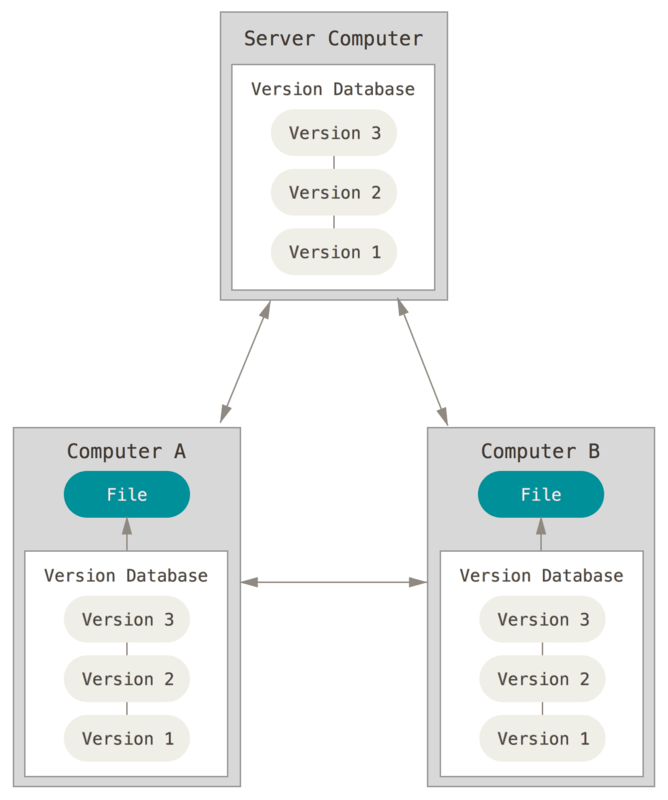
\includegraphics[width=0.4\textwidth]{paper-images/distributed.png}
\caption{Chacon \& Straub (2014) Distributed version control.} 
\label{fig:distributed-vcs}
\end{figure}

Git includes a specialized algorithm to automatically merge new changes into the code base. Consequentially, the consensus problem is often automatically solved. However, when two developers made changes to the same code, the algorithm fails, resulting in a ``merge conflict''. It is then up to the developers to manually solve the conflict. 

Immutability is not enforced in git. This means that any developer can manipulate the history of changes. This is useful when, for example, a large file has accidentally been included into the project. This bloats the size of the project and hampers collaboration. Simply removing the file does not help, as the file will still be part of the code history. To completely get rid of this file, the original inclusion has to be nullified. However, this could be used for malicious practices as well. Imagine a problem arises because of a programming mistake a developer made some weeks ago. In case the developer does not want to be held accountable, he could remove his change from the history. Or he could even change the author of the change to someone else \cite{change-author-commit}.

It is clear that the git system needs trust between the developers. But in some projects, there is no trust. For example, in open source projects, any developer can propose code changes. This is why on hosting sites for git repositories, such as Github, authorized users need to approve a code change before it can be added to the main code base \cite{github-pr}. But this partially removes the distributed character of git.

Considering the CAP theorem, git is available and partition-resilient, but not consistent. A node can always download a version of the code base, either from the main server or from one of its colleagues. This makes git available. If a node goes offline, a developer can contact any other developer for the full code base, making git partition-resilient. However, as every developer has a slightly different code base because of his own changes, git will never be consistent.

\subsubsection{BitTorrent}

BitTorrent is a peer-to-peer file distribution system. Instead of downloading a file from a central server, users download the file from peers that already (partially) have the file. Once a file is uploaded with BitTorrent, it can no longer be changed. Most databases need some sort of write functionality. This characteristic disqualifies BitTorrent for most database applications. Yet, the single focus makes BitTorrent work really well for file sharing. As a result, BitTorrent was one of the first widely accepted collaborative, distributed networks. It ``increasingly becomes the norm for media acquisition among the general Internet public'' (Andersson, J. 2009 \cite{bittorrent-norm})

As there are no updates to a BitTorrent file, consensus and immutability are not an issue. Also, the CAP theorem is not relevant in this writeless context. BitTorrent is consistent, available and partition-resilient.

\subsubsection{Blockchain}
\label{subsubsec:blockchain-as-distributed-dbs}
\iffalse
- CAP Theorem
 => maybe add a section about database properties in general (CAP theorem) and the blockchain aspect of it (one of the papers mentions this, I think Bitfury)
- general advantages of blockchains as a database: consistency and consensus 
- disadvantages of blockchains: latency and scalability
\fi

Blockchain technology has already been explained in the previous section. Blockchain solves both the consensus issue as the immutability issue quite well. Therefore, it is a prime candidate for applications that require a collaborative database.

% consensus: forks and resolving
Blockchain handles the consensus issue quite well. As previously explained, once a miner has found a new valid block, he propagates this block through the blockchain network. Other miners will continue mining on the new block, appending the blockchain. But if two miners simultaneously find a valid block, they will both propagate this block through the network. Some miners will first receive one block and continue mining on top of that block, others will mine on top of the other block. Now, there are effectively two different versions of the database. This phenomenon is called a fork. To solve this fork, miners are incentivized to work on top of the longest fork. As it is unlikely that miners will again simultaneously find a new valid block, one fork will quickly become longer than the other. This compels the miners to switch to the longest fork, thus resolving the fork \cite{antonopoulos:2014}. 

% TODO consistency: incredibly hard to rewrite history, as would need to recalculate all the blocks afterward

Immutability is built into the blockchain idea. An attacker would first have to create a fork before a certain block he wants to alter. For this fork to be accepted as the proper blockchain, the attacker would need to make the fork longer than the current blockchain. Considering a proof of work consensus mechanism, without more than 50\% of the network's computing power, this is mathematically impossible for blocks deep in the blockchain. As Nakamoto (2008) calculates in his paper, there is less than 0.1\% an attacker with 25\% of total computing power can catch up after 15 blocks have passed. As currently, the largest mining pool holds only 23.8\% \cite{hashrate-distribution}, waiting 15 blocks would be extremely safe. In general, the bitcoin community agrees that after 6 confirmation blocks a transaction is confirmed \cite{bitcoin-confirmation-amount}. For small transactions, best practice states that one confirmation block should suffice. Larger transactions might need three confirmation blocks \cite{confirmation-safety}.

% TODO cap: ap and eventually consistent: 

The CAP theorem can also be applied to blockchains. As Goland states in his blog \cite{blockchain-cap}, blockchains are available and partition-resilient and eventually consistent. As said before concerning the bitcoin blockchain, a user can be virtually sure that a block is immutable after 6 confirmation blocks \cite{bitcoin-confirmation-amount}.

However, there are some practical disadvantages with the blockchain. The first disadvantage is the lack of scalability of a blockchain. The main reason is that blockchain holds all transactions ever executed. As a result, the size of the blockchain constantly increases. This gradually pushes smaller nodes out of the network as they cannot afford to hold the entire blockchain in storage \cite{blockchain-scalability}. Another disadvantage is the latency of blockchains. To make sure a transaction has been included in the blockchain, merchants are expected to wait for some confirmation blocks. For example, the bitcoin blockchain creates one block every 10 minutes. This could be is an issue for several applications. Imagine going to a coffee shop and having to wait 30 minutes before you can get your coffee. Even though there are blockchains with lower block time (ethereum has a block time of 22 seconds \cite{ethereum-block-time}), these blockchains need more confirmations because of the higher chance of a fork. Another important concern concerning public blockchains could be privacy. Although the data stored to the blockchain can be properly encrypted, everyone with reading access to the blockchain can see when this data is submitted. Finally, some applications might require delete functionality. Because of blockchain's immutability, data can never be deleted.

\subsubsection{Non-persistent P2P networks}

The final aspect of this chapter discusses collaborative peer-to-peer (P2P) networks that are not persistent. This means that the data on the network is not stored. It can only be accessed in real-time. 

An example of such a network is Open Bazaar. Open bazaar is a decentralized peer-to-peer marketplace. When a customer buys an item from eBay, the customer searches through listings that have been posted to the centralized servers of eBay. When searching for a specific item on Open Bazaar, a customer searches through the network of nodes that are currently online. But when a node posting a listing goes offline, this listing will no longer show up in search results \cite{openbazaar-faq}. This is why we call this a non-persistent network instead of a distributed database.

\iffalse
- no cap applicable, as not a database
- examples: open bazaar.
\fi

